\section{User Workflow}

The steps that a user of the application will follow are detailed in this section.

\begin{figure}[H]
    \centering
	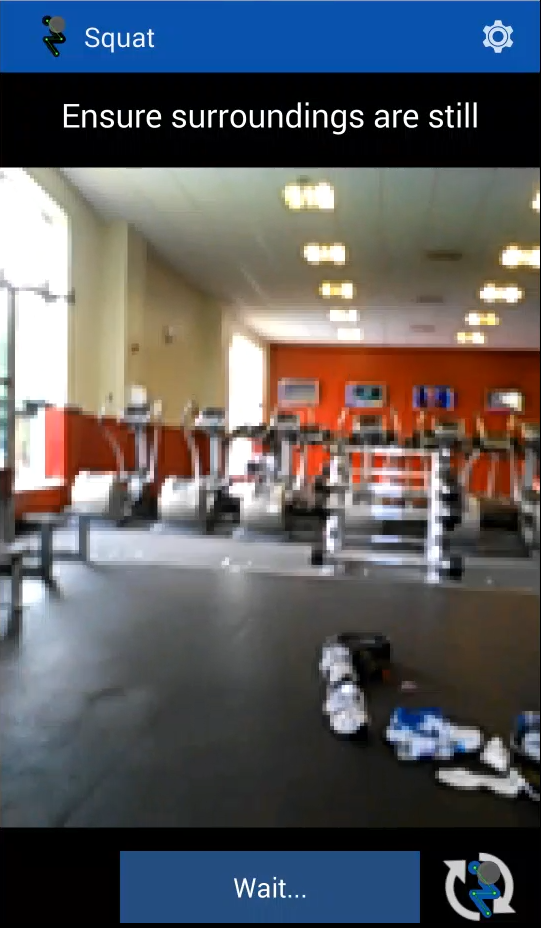
\includegraphics[height=10cm]{application/images/ensuresurroundingsstill}
\caption{Wait until the device and its surroundings are still}
\label{fig:ensuresurroundings}
\end{figure}

The user begins by starting up the application. They will immediately see a video feed of the front-facing camera of their Android mobile device. They will see a message at the top of the screen, instructing them in the first step they must take: `Ensure surroundings are still.

A button at the bottom of the screen displays the text `Wait...', indicating that some action must be performed before the button can be pressed. Figure~\ref{fig:ensuresurroundings} shows this screen.

\begin{figure}[H]
    \centering
	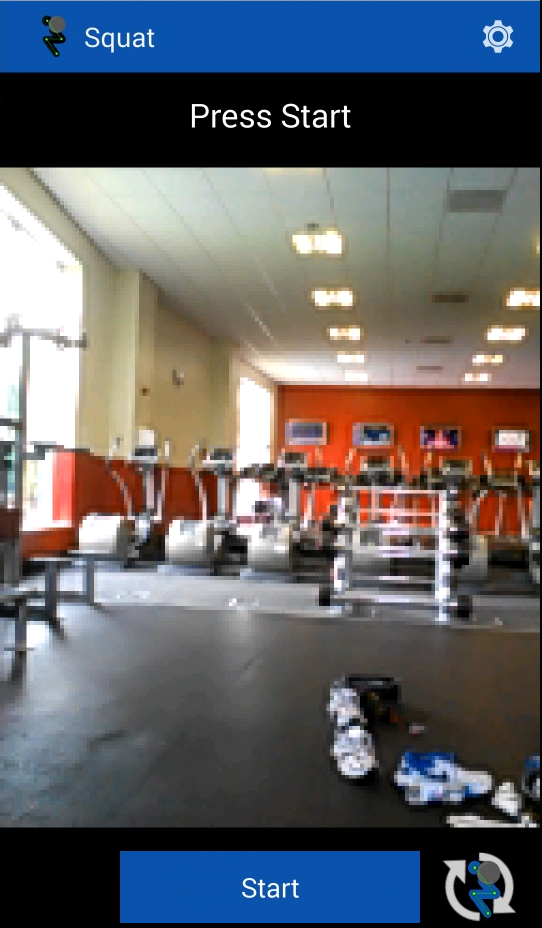
\includegraphics[height=10cm]{application/images/pressstart}
\caption{The background is deemed still, allow the user to press start}
\label{fig:pressstart}
\end{figure}

As the user follows the on-screen instruction of ensuring that their surroundings are still, they will notice that the instruction text changes to `Press Start' automatically, and the button displays `Start' and is lightened to indicate that it may be pressed. This screen is shown in figure~\ref{fig:pressstart}.

This initial stage of disabling and enabling the button ensures that the user places their phone in a location where it will not move, to allow background subtraction to work effectively. It also ensures that there is no movement in the background, which may distort the background subtraction and cause the model to `lock on' to a different figure.

The application tolerates a little movement, meaning that movement too far away to cause background subtraction issues is allowed. This avoids the frustration of a user requiring an area completely devoid of movement to use the application.

\begin{figure}[H]
    \centering
	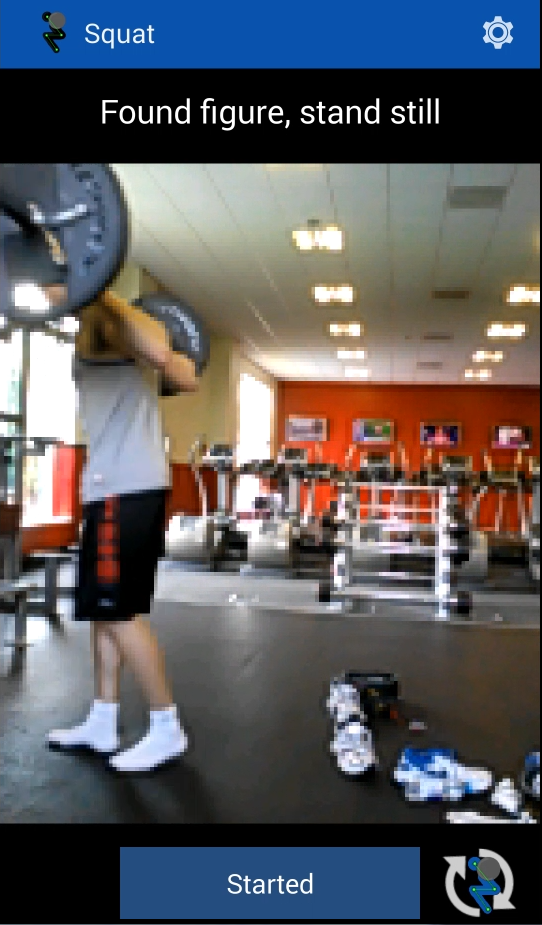
\includegraphics[height=10cm]{application/images/foundfigure}
\caption{A figure has been detected}
\label{fig:foundfigure}
\end{figure}

As a side note, there is also a button to the right of the start button. This button is used to flip the expected orientation of the lifter. It defaults to expect the lifter to face left (as they look at the screen). When this button is pressed, the figure in the icon flips to indicate that the lifter must stand facing the opposite direction. Vocal feedback is also used, with a voice saying `Face left.' or `Face right.' to confirm this change of orientation.

Once the start button is enabled, the user presses the button, and immediately receives vocal directions to `Walk into view and stand still, facing left', as well as the instruction text changing to `Walk into view'. The vocal instruction here will say `Walk into view and stand still, facing right' should the orientation have been changed by the user.

The user will follow these instructions, collecting their barbell from the squat rack out of view, and walking into the application's view. As the user walks into view, the instruction text will update to indicate that the user has been recognised by the application: `Found figure, stand still'. This is shown in figure~\ref{fig:foundfigure}.

\begin{figure}[H]
    \centering
	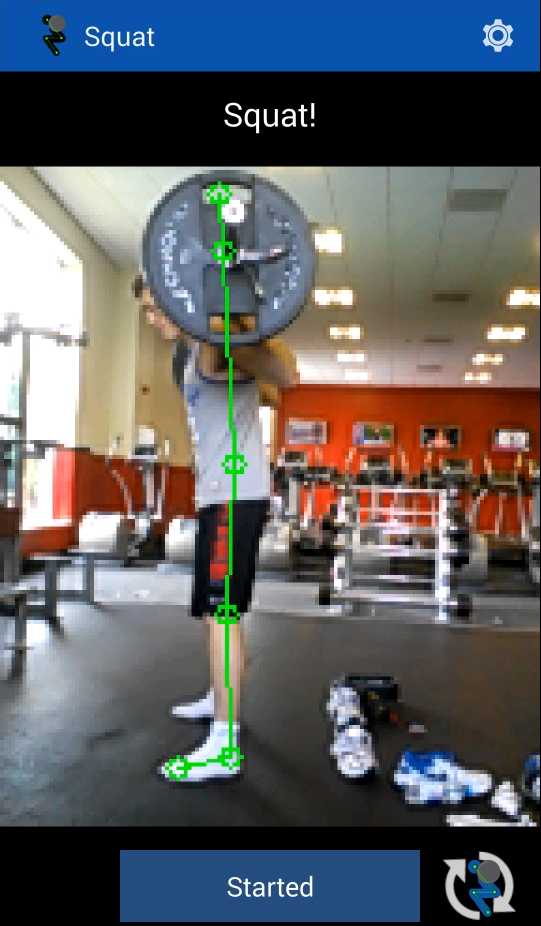
\includegraphics[height=10cm]{application/images/startsquatting}
\caption{The model is mapped to the figure once the figure is still}
\label{fig:startsquatting}
\end{figure}

Once the user has moved into position, and stood still following the instructions, the application will emit a beep as it fits the initial model to the user. As it does this, the video feed will add an overlay showing the model drawn as a skeleton - with lines connecting points in a stick figure fashion. Although this is not the model drawing method used in fitting, it is more intuitive for the user to see a skeleton view than the model constructed of ellipses. This encapsulates the underlying functionality, displaying the model in a user-friendly way. From this, the user can see that they have been recognised by the application, and that the application has started to track their movement. Figure~\ref{fig:startsquatting} shows this stage.

\begin{figure}[H]
    \centering
	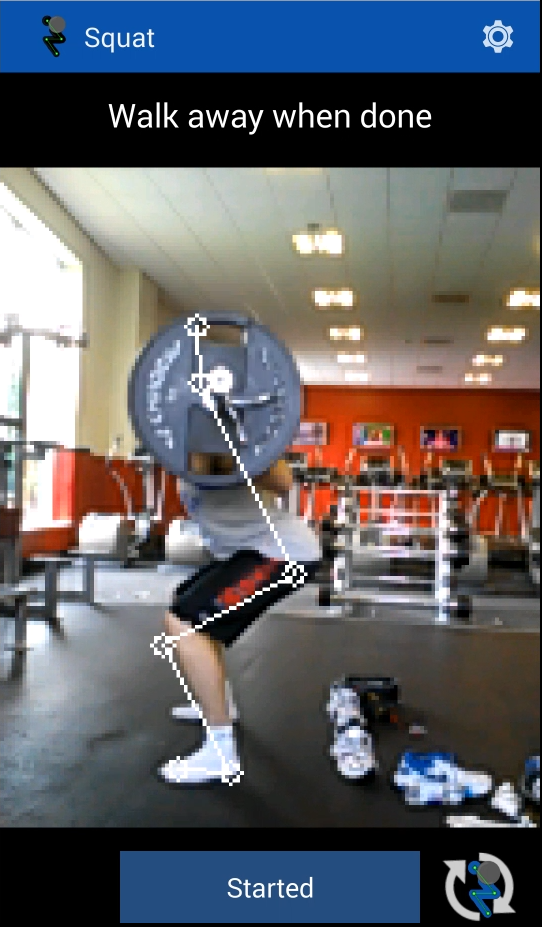
\includegraphics[height=10cm]{application/images/midsquat}
\caption{The skeleton tracks the lifter's movement throughout the squatting phase}
\label{fig:midsquat}
\end{figure}

As the model is displayed and the application beeps, the application's voice will indicate the next move expected from the user by saying `Start squatting when ready'. The user may now begin squatting in their own time. As they squat, the skeleton on screen will be updated in real-time as the tracking part of the algorithm runs, as shown in figure~\ref{fig:midsquat}.

\begin{figure}[H]
    \centering
	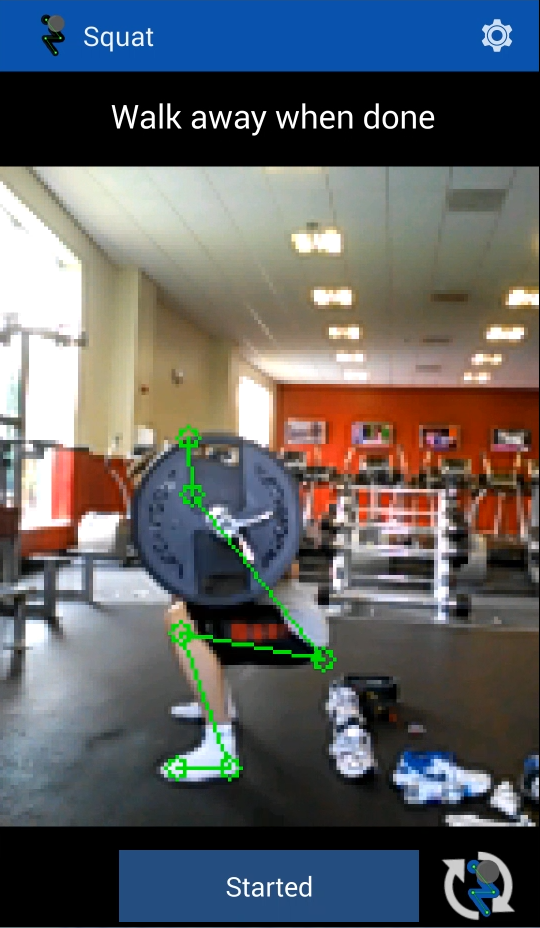
\includegraphics[height=10cm]{application/images/belowparallel}
\caption{The skeleton is drawn in green to indicate that the squat is low enough}
\label{fig:belowparallel}
\end{figure}

As the user descends low enough for the squat to be considered valid, the application emits another beep. This real-time feedback is incredibly useful, meaning that the user will know when they have squatted low enough during the movement, rather than only discovering this after they have finished their set. When hearing a beep, the user knows immediately that they must start the ascension part of the movement and can begin to drive with their legs. On-screen, the skeleton changes colour to green (as shown in figure~\ref{fig:belowparallel}), reinforcing the notion that their squat is low enough to be considered valid.

\begin{figure}[H]
    \centering
	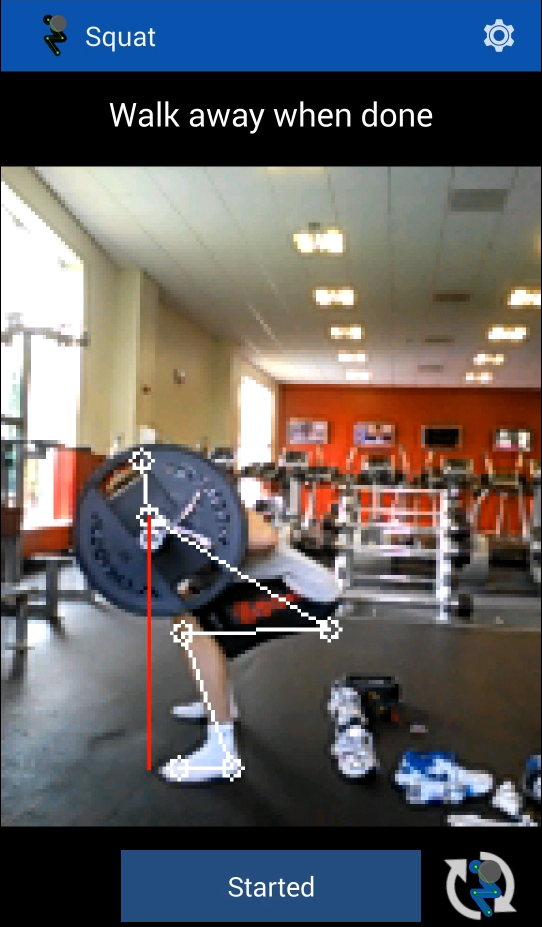
\includegraphics[height=10cm]{application/images/weightdistro}
\caption{A red line indicates sub-optimal weight distribution}
\label{fig:weightdistro}
\end{figure}

Another element of visual feedback is a line which shows the weight distribution of the squat. For a squat to be optimal, the bar must be directly above the feet at all times, giving the user maximum leverage to support the weight. Should the application detect that this is not the case and the weight is too far in front of the lifter's toes, or too far behind the lifter's heels, a red vertical line is drawn from the bar to the feet, as shown in figure~\ref{fig:weightdistro}. This traces the weight's position above the feet, showing that it is too far forward or backward.

\begin{figure}[H]
    \centering
	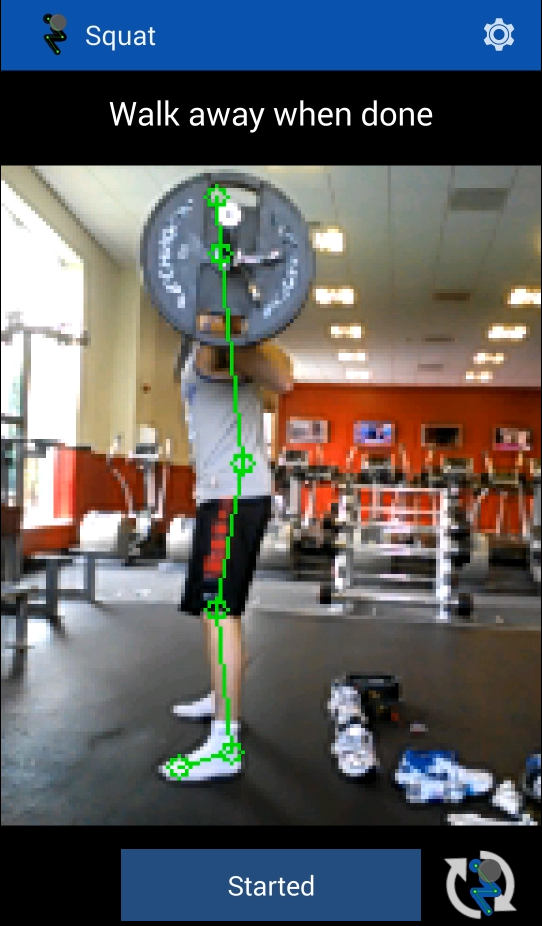
\includegraphics[height=10cm]{application/images/lockout}
\caption{The skeleton is drawn in green and vocal feedback is given as the lifter locks out}
\label{fig:lockout}
\end{figure}

As the user completes the ascension part of the squat (thus completing one full repetition) and `locks out', the skeleton is again coloured green as shown in figure~\ref{fig:lockout}. At this point, the application detects that a repetition has been completed, and provides the user with vocal feedback. This vocal feedback includes the current rep number, how successful the squat was, and a tip on how to improve the squat if necessary. An example might be `Two. Good. Try leaning forward a little more.', or `Four. Ok. Try squatting deeper.'.

So as not to bore the user with the same repetitive messages, slight variations of each tip are chosen at random, depending on the main problem with the squat. For example if the user fails to squat deep enough, they may be told to `Squat deeper.' or `Try to squat below parallel' or one of many other variations.

The part of the feedback which tells the user how well their squat was performed overall can be one of the following: `Not very good.', `Ok.', `Good.', `Very good.', `Excellent', `Perfect'. These are selected based on the score for the rep that they have just completed. For example, `Very good.' is said should the user achieve a score between 70\% and 90\%. When a user achieves a score above 90\%, the verbal feedback will not provide the user with a tip. This gives the user a more satisfying experience, encouraging the user to strive towards good squatting technique.

The full range of vocal feedback is detailed in the appendix (section~\ref{sec:appendix_feedback}).

\begin{figure}[H]
    \centering
	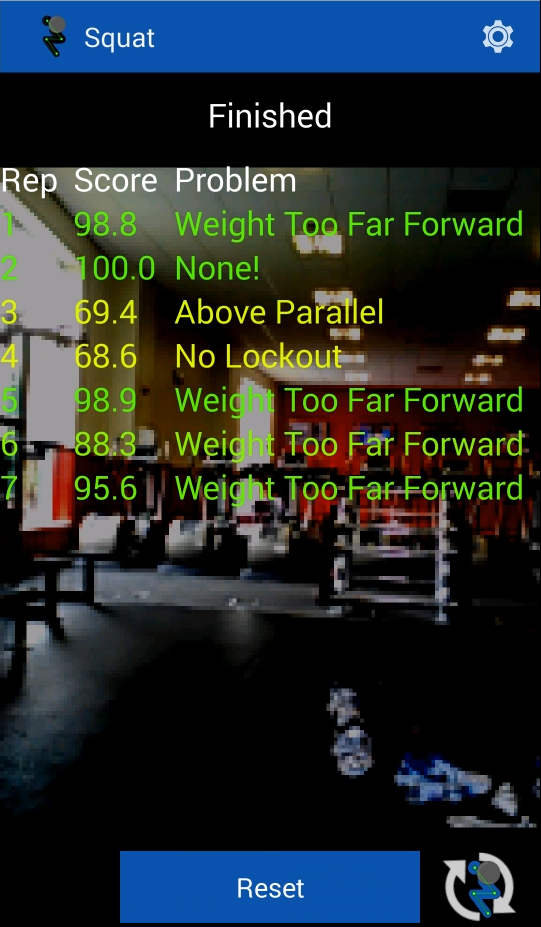
\includegraphics[height=10cm]{application/images/scores}
\caption{The lifter's scores are displayed once they have finished squatting}
\label{fig:scores}
\end{figure}

This process repeats for every repetition completed by the user. Feedback is given as the figure is detected to stand up straight or, should they fail to fully lock out, as they begin descending into their next repetition.

When the user has completed their desired number of squats, they simply walk out of view. This follows the usual procedure, where a lifter will place the weight back in the rack on the completion of their set of squats. As they walk away, the tracking and analysis phase will end, and a breakdown of their scores is displayed on the screen as shown in figure~\ref{fig:scores}.



Here, the user can see their score for each repetition they completed, and also the main `problem' with their squat. Each entry in the table is coloured in relation to its score, giving the user an instant visual indication as to how well their squat was performed, without the need to read each score value. A set of scores that is mostly green will indicate to the user that they performed a good set of squats, and a largely orange or red set of scores will inform the user that they should improve their technique.

Once the user has reviewed their scores, they can press the reset button. This will change the application to its initial state, allowing the user to press the start button once their surroundings are still.